\documentclass[12pt, a4paper]{report}
\usepackage{epsfig}
\usepackage{subfigure}
%\usepackage{amscd}
\usepackage{amssymb}
\usepackage{graphicx}
%\usepackage{amscd}

\usepackage{subfiles}
\usepackage{framed}
\usepackage{subfiles}
\usepackage{amsthm, amsmath}
\usepackage{amsbsy}
\usepackage{framed}
\usepackage[usenames]{color}
\usepackage{listings}
\lstset{% general command to set parameter(s)
	basicstyle=\small, % print whole listing small
	keywordstyle=\color{red}\itshape,
	% underlined bold black keywords
	commentstyle=\color{blue}, % white comments
	stringstyle=\ttfamily, % typewriter type for strings
	showstringspaces=false,
	numbers=left, numberstyle=\tiny, stepnumber=1, numbersep=5pt, %
	frame=shadowbox,
	rulesepcolor=\color{black},
	columns=fullflexible
} %
%\usepackage[dvips]{graphicx}
\usepackage{natbib}
\bibliographystyle{chicago}
\usepackage{vmargin}
% left top textwidth textheight headheight
% headsep footheight footskip
\setmargins{3.0cm}{2.5cm}{15.5 cm}{22cm}{0.5cm}{0cm}{1cm}{1cm}
\renewcommand{\baselinestretch}{1.5}
\pagenumbering{arabic}
%\theoremstyle{plain}
\newtheorem{theorem}{Theorem}[section]
\newtheorem{corollary}[theorem]{Corollary}
\newtheorem{ill}[theorem]{Example}
\newtheorem{lemma}[theorem]{Lemma}
\newtheorem{proposition}[theorem]{Proposition}
\newtheorem{conjecture}[theorem]{Conjecture}
\newtheorem{axiom}{Axiom}
\theoremstyle{definition}
\newtheorem{definition}{Definition}[section]
\newtheorem{notation}{Notation}
\theoremstyle{remark}
\newtheorem{remark}{Remark}[section]
\newtheorem{example}{Example}[section]
\renewcommand{\thenotation}{}
%\renewcommand{\thetable}{\thesection.\arabic{table}}
%\renewcommand{\thefigure}{\thesection.\arabic{figure}}

\author{ } \date{ }

\begin{document}
%\tableofcontents


%In this section, we introduce the LME model, discusss how it can be applied to method comparison problems, and how it is desirable in the case of replicate measurements, giving some examples from previous work (i.e. Carstensen et Al, Lai \& Shaio, and Roy). Further to that, there will be a demonstration on fitting various types LME models using freely available software.
%
%\subsection{Conclusion}
%\citet{BXC2008} and \citet{ARoy2009} highlight the need for method comparison methodologies suitable for use in the presence of replicate measurements. \citet{ARoy2009} presents a comprehensive methodology for assessing the agreement of two methods, for replicate measurements. This methodology has the added benefit of overcoming the problems of unbalanced data and unequal numbers of replicates. Implementation of the methodology, and interpretation of the results, is relatively easy for practitioners who have only basic statistical training. Furthermore, it can be shown that widely used existing methodologies, such as the limits of agreement, can be incorporated into Roy's methodology.
%
%
%  

\chapter{Linear Mixed Effects Models}
While the method comparison problem is conventionally poised in the context of two methods of measurements, LME models allow for a straightforward analysis whereby several methods of measurement can be measured simulataneously. However simple models can only indicate agreement of lack thereof, and the presence of inter-method bias. To consider more complex questions, more complex LME models would be required.

Linear mixed effects (LME) models can facilitate greater understanding of the potential causes of bias and differences in precision between two sets of measurement. Due to computation complexity, LME models have not seen widespread use until many well known statistical software applications began facilitating them. Consequently LME approaches have seen increased use as a framework for method comparison studies in recent years (Lai $\&$ Shaio, \citet{BXC2004,BXC2008} and \citet{ARoy2009} as examples), due to a higher profile in scientific literature, and the increased availability of capable software. Additionally development of a framework for LME model diagnostics has progressed, thanks to authors such as \citet{schabenberger}, \citet{Christensen}, \citet{cook86} \citet{west}, amongst others.

\section{Linear Mixed Effects Models}
A linear mixed effects (LME) model is a statistical model containing both fixed effects and random effects (also known as variance components). LME models are a generalization of the classical linear model, which contain fixed effects only. When the levels of factors are considered to be sampled from a population, and each level is not of particular interest, they are considered random quantities with associated variances.

The effects of the levels, as described, are known as random effects. Random effects are represented by unobservable normally distributed random variables. Conversely fixed effects are considered non-random and the levels of each factor are of specific interest.
%LME models are useful models when considering repeated measurements or grouped observations.

\citet{Fisher4} introduced variance components models for use in genetical studies. Whereas an estimate for variance must take an non-negative value, an individual variance component, i.e.\ a component of the overall variance, may be negative.

The methodology has developed since, including contributions from
\citet{tippett}, who extend the use of variance components into linear models, and \citet{eisenhart}, who introduced the `mixed model' terminology and formally distinguished between mixed and random effects models. \citet{Henderson1950} devised a methodology for deriving estimates for both the fixed effects and the random effects, using a set of equations that would become known as `mixed model equations' or `Henderson's equations'.
LME methodology is further enhanced by Henderson's later works \citep{Henderson53, Henderson59,Henderson63,Henderson73,Henderson84a}. The key features of Henderson's work provide the basis for the estimation techniques.

\citet{HartleyRao} demonstrated that unique estimates of the variance components could be obtained using maximum likelihood methods. However these estimates are known to be biased `downwards' (i.e. underestimated), because of the assumption that the fixed estimates are known, rather than being estimated from the data. \citet{PT71} produced an alternative set of estimates, known as the restricted maximum likelihood (REML) estimates, that do not require the fixed effects to be known. 

Thusly there is a distinction the REML estimates and the original estimates, now commonly referred to as ML estimates.

\subsection{Laird-Ware Model} 
\citet{LW82} provides a form of notation for notation for LME models that has since become the standard form, or the basis for more complex formulations. Due to computation complexity, linear mixed effects models have not seen widespread use until many well known statistical software applications began facilitating them. SAS Institute added PROC MIXED to its software suite in 1992 \citep{singer}. \citet{PB} described how to compute LME models in the \texttt{S-plus} environment.

Linear mixed effects models (LME)
differs from the conventional linear model in that it has both
fixed effects and random effects regressors, and coefficients
thereof. The notation provided here is generic, and will be adapted to accord with complex formulations that will be encountered in due course. Using Laird-Ware form, the LME model is commonly described in matrix form,
\begin{equation}
Y = X\beta + Zb + \epsilon
\label{LW}
\end{equation}

Y is the $n \times 1$ response vector, where  $n$ is the number of observations. \textit{$\beta$} is a $p \times 1$ vector of fixed $p$ effects, with the
first element being the population mean. $X$ and $Z$ are $n \times p$ and $n \times q$ ``model matrices`` for fixed effects and random effects respectively, comprising
$0$s or $1$s, depending on the observation is question. The vector of residuals, v(\textit{e}) has
dimension $n \times 1$. The random effects are contained in the  $q \times
1$ vector \textit{b}.

%\subsection{ (good)Likelihood and estimation}

% Likelihood is the hypothetical probability that an event that has already occurred would yield a specific outcome. Likelihood differs from probability in that probability refers to future occurrences, while likelihood refers to past known outcomes.

% The likelihood function ($L(\theta)$)is a fundamental concept in statistical inference. It indicates how likely a particular population is to produce an observed sample. The set of values that maximize the likelihood function are considered to be optimal, and are used as the estimates of the parameters. For computational ease, it is common to use the logarithm of the likelihood function, known simply as the log-likelihood ($\ell(\theta)$).

\subsection{LME Model Estimation}
Estimation of LME models involve two complementary estimation issues'; estimating the vectors of the fixed and random effects estimates $\hat{\beta}$ and $\hat{b}$ and estimating the variance covariance matrices $G$ and $\Sigma$. Inference about fixed effects have become known as `estimates', while inferences about random effects have become known as `predictions'. The most common approach to obtain estimators are Best Linear Unbiased Estimator (BLUE) and Best Linear Unbiased Predictor (BLUP). For an LME model given by (\ref{LW}), the BLUE of $\hat{\beta}$ is given by
\begin{equation}
\hat{\beta} = (X^\prime V^{-1}X)^{-1}X^\prime V^{-1}y,
\end{equation}whereas the BLUP of $\hat{b}$ is given by
\begin{equation}
\hat{b} = DZ^{\prime} V^{-1} (y-X\hat{\beta}).
\end{equation}
\subsubsection{Henderson's Equations}
Because of the dimensionality of V (i.e. $n \times n$) computing the inverse of V can be difficult. As a way around the this problem \citet{Henderson53, Henderson59,Henderson63,Henderson73,Henderson84a} offered a more simpler approach of jointly estimating $\hat{\beta}$ and $\hat{b}$.
\cite{Henderson:1950} made the (ad-hoc) distributional assumptions $y|b \sim \mathrm{N} (X \beta + Zb, \Sigma)$ and $b \sim \mathrm{N}(0,D),$ and proceeded to maximize the joint density of $y$ and $b$
\begin{equation}
\left|
\begin{array}{cc}
G & 0 \\
0 & \Sigma \\
\end{array}
\right|^{-\frac{1}{2}}
\exp
\left\{ -\frac{1}{2}
\left(
\begin{array}{c}
b \\
y - X \beta -Zb \\
\end{array}
\right)^\prime
\left( \begin{array}{cc}
G & 0 \\
0 & \Sigma \\
\end{array}\right)^{-1}
\left(
\begin{array}{c}
b \\
y - X \beta -Zb \\
\end{array}
\right)
\right\},
\label{u&beta:JointDensity}
\end{equation}
with respect to $\beta$ and $b,$ which ultimately requires minimizing the criterion
\begin{equation}
(y - X \beta -Zb)'\Sigma^{-1}(y - X \beta -Zb) + b^\prime D^{-1}b.
\label{Henderson:Criterion}
\end{equation}
This leads to the mixed model equations
\begin{equation}
\left(\begin{array}{cc}
X^\prime\Sigma^{-1}X & X^\prime\Sigma^{-1}Z
\\
Z^\prime\Sigma^{-1}X & X^\prime\Sigma^{-1}X + G^{-1}
\end{array}\right)
\left(\begin{array}{c}
\beta \\
b
\end{array}\right)
=
\left(\begin{array}{c}
X^\prime\Sigma^{-1}y \\
Z^\prime\Sigma^{-1}y
\end{array}\right).
\label{Henderson:Equations}
\end{equation}
Using these equations, obtaining the estimates requires the inversion of a matrix
of dimension $p+q \times p+q$, considerably smaller in size than $V$. \citet{Henderson63} shows that these mixed model equations do not depend on normality and that $\hat{\beta}$ and $\hat{b}$ are the BLUE and BLUP under general conditions, provided $G$ and $\Sigma$ are known.

\cite{Robi:BLUP:1991} points out that although \cite{Henderson:1950} initially referred to the estimates $\hat{\beta}$ and $\hat{b}$ from (\ref{Henderson:Equations}) as ``joint maximum likelihood estimates", \cite{Henderson:1973} later advised that these estimates should not be referred to as ``maximum likelihood" as the function being maximized in (\ref{Henderson:Criterion}) is a joint density rather than a likelihood function. \cite{YLee} remarks that it is clear that Henderson used joint estimation for computational purposes, without recognizing the theoretical implications.

%========================================================================================%

\subsubsection{Estimation of the Fixed Parameters}

The vector $y$ has marginal density $y \sim \mathrm{N}(X \beta,V),$ where $V = \Sigma + ZDZ^\prime$ is specified through the variance component parameters $\theta.$ The log-likelihood of the fixed parameters $(\beta, \theta)$ is
\begin{equation}
\ell (\beta, \theta|y) =
-\frac{1}{2} \log |V| -\frac{1}{2}(y -
X \beta)'V^{-1}(y -
X \beta), \label{Likelihood:MarginalModel}
\end{equation}
and for fixed $\theta$ the estimate $\hat{\beta}$ of $\beta$ is obtained as the solution of
\begin{equation}
(X^\prime V^{-1}X) {\beta} = X^\prime V^{-1}y.
\label{mle:beta:hat}
\end{equation}

Substituting $\hat{\beta}$ from (\ref{mle:beta:hat}) into $\ell(\beta, \theta|y)$ from (\ref{Likelihood:MarginalModel}) returns the \emph{profile} log-likelihood
\begin{eqnarray*}
\ell_P(\theta \mid y) &=& \ell(\hat{\beta}, \theta \mid y) \\
&=& -\frac{1}{2} \log |V| -\frac{1}{2}(y - X \hat{\beta})'V^{-1}(y - X \hat{\beta})
\end{eqnarray*}
of the variance parameter $\theta.$ Estimates of the parameters $\theta$ specifying $V$ can be found by maximizing $\ell_P(\theta \mid y)$ over $\theta.$ These are the ML estimates. For REML estimation the \emph{restricted} log-likelihood is defined as
\[
\ell_R(\theta \mid y) =
\ell_P(\theta \mid y) -\frac{1}{2} \log |X^\prime VX |.
\]
%\subsubsection{ (good)Likelihood estimation techniques}
%Maximum likelihood and restricted maximum likelihood have become the most common strategies
%for estimating the variance component parameter $\theta.$ Maximum likelihood estimation obtains
%parameter estimates by optimizing the likelihood function.
%To obtain ML estimate the likelihood is constructed as a function of the parameters in the specified LME model.
% The maximum likelihood estimates (MLEs) of the parameters are the values of the arguments that maximize the likelihood function.

The REML approach does not base estimates on a maximum likelihood fit of all the information, but instead uses a likelihood function derived from a data set, transformed to remove the irrelevant influences \citep{REMLDefine}. Restricted maximum likelihood is often preferred to maximum likelihood because REML estimation reduces the bias in the variance component by taking into account the loss of degrees of freedom that results from estimating the fixed effects in ${\beta}$. Restricted maximum likelihood also handles high correlations more effectively, and is less sensitive to outliers than maximum likelihood.  The problem with REML for model building is that the likelihoods obtained for different fixed effects are not comparable. Hence it is not valid to compare models with different fixed effects using a likelihood ratio test or AIC when REML is used to estimate the model. Therefore models derived using ML should be used instead.

\subsubsection{Estimation of the Random Effects}

The established approach for estimating the random effects is to use the best linear predictor of $b$ from $y,$ which for a given $\beta$ equals $GZ^\prime V^{-1}(y - X \beta).$ In practice $\beta$ is replaced by an estimator such as $\hat{\beta}$ from (\ref{mle:beta:hat}) so that $\hat{b} = DZ^\prime V^{-1}(y - X \hat{\beta}).$ Pre-multiplying by the appropriate matrices it is straightforward to show that these estimates $\hat{\beta}$ and $\hat{b}$ satisfy the equations in (\ref{Henderson:Equations}).

%\subsubsection{Estimation of Fixed and Random Effects}
%Potentially it may be impossible to compute unique BLUE estimates for all the fixed factors in a model. This may be due to linear dependence in the model
%matrix \textbf{X}. 
%
%Estimation of random effects for LME models in the NLME package is accomplished through use
%of both EM (Expectation-Maximization) algorithms and Newton-Raphson algorithms.
%\begin{itemize}
%\item EM iterations bring estimates of the parameters into the region of the optimum very quickly, but
%convergence to the optimum is slow when near the optimum.
%\item Newton-Raphson iterations are computationally intensive and can be unstable when far from the
%optimum. However, close to the optimum they converge quickly.
%\item The LME function implements a hybrid approach, using 25 EM iterations to quickly get near the
%optimum, then switching to Newton-Raphson iterations to quickly converge to the optimum. \item If
%convergence problems occur, the ``control” argument in LME can be used to change the way the
%model arrives at the optimum.
%\end{itemize}
%





%\subsubsection{Likelihood and estimation}
%Likelihood is the hypothetical probability that an event that has
%already occurred would yield a specific outcome. Likelihood
%differs from probability in that probability refers to future
%occurrences, while likelihood refers to past known outcomes.
%
%
%Likelihood functions provide the basis for two important statistical concepts that shall be further referred to; the likelihood ratio test and the Akaike information criterion. The likelihood function, $L(\theta)$, is a fundamental concept in statistical
%inference. It indicates how likely a particular population is to produce an observed sample. The set of values that maximize the
%likelihood function are considered to be optimal, and are used as the estimates of the parameters. For computational ease, it is common to use the logarithm of the likelihood function, known simply as the log-likelihood ($\ell(\theta)$).
%
%Assuming a statistical model $f_{\theta}(y)$ parameterized by a fixed and unknown set of parameters $\theta$, the likelihood $L(\theta)$ is the probability of the observed data $y$ considered as a function of $\theta$ \citep{YLee}.
%
%\subsubsection{Likelihood-based tools}
%The maximum likelihood estimates (MLEs) of the parameters are the values of the arguments that maximize the likelihood function. Maximum likelihood and restricted maximum likelihood have become the most common strategies for estimating the variance component parameter $\theta.$ Maximum likelihood (ML) estimation is a well known method of
%obtaining estimates of unknown parameters by optimizing a likelihood function.  To obtain ML estimate the likelihood is constructed as a function of the parameters in the specified LME model. 
%
%Thelikelihood function is constructed as a function of the parameters
%in the specified model. Models fitted by ML estimation can be compared using the likelihood ratio test. However ML is known to underestimate variance components for finite samples \citep{Demi}. 





%%%%%%%%%%%%%%%%%%%%%%%%%%%%%%%%%%%%%%%%%%%%%%%%%%%%%%%%%%%%%%%%%%%%%%%%%%%%%%%% ML and REML

\subsubsection{Algorithms for Likelihood Function Optimization}

Iterative numerical techniques are used to optimize the log-likelihood function and estimate the covariance parameters $\theta$. The procedure is subject to the constraint that $R$ and $G$ are both positive definite. The most common iterative algorithms for optimizing the likelihood function are the Newton-Raphson method, which is the preferred method, the expectation maximization (EM) algorithm and the Fisher scoring methods.

The EM algorithm, introduced by \citet{EM}, is an iterative technique for maximizing complicated likelihood functions. The algorithm alternates between performing an expectation (E) step and the maximization (M) step. The `E' step computes the expectation of the log-likelihood evaluated using the current estimate for the variables. In the `M' step, parameters that maximize the expected log-likelihood, found on the previous `E' step, are computed. These parameter estimates are then used to determine the distribution of the variables in the next `E' step. The algorithm alternatives between these two steps until convergence is reached.

The main drawback of the EM algorithm is its slow rate of convergence. Consequently the EM algorithm is rarely used entirely in LME estimation, instead providing an initial set of values that can be passed to other optimization techniques.

The Newton-Raphson (NR) method is the most common, and recommended technique for ML and REML estimation. The NR algorithm minimizes an objective function defines as $-2$ times the log likelihood for the covariance parameters $\theta$. At every iteration the NR algorithm requires the calculation of a vector of partial derivatives, known as the gradient, and the second derivative matrix with respect to the covariance parameters. This is known as the observed Hessian matrix. Due to the Hessian matrix, the NR algorithm is more time-consuming, but convergence is reached with fewer iterations compared to the EM algorithm. The Fisher scoring algorithm is an variant of the NR algorithm that is more numerically stable and likely to converge, but not recommended to obtain final estimates.

\subsubsection{The Extended Likelihood}

The desire to have an entirely likelihood-based justification for estimates of random effects, in contrast to Henderson's equation, has motivated \citet[page 429]{Pawi:in:2001} to define the \emph{extended likelihood}. He remarks ``In mixed effects modelling the extended likelihood has been called \emph{h-likelihood} (for hierarchical  likelihood) by \cite{Lee:Neld:hier:1996}, while in smoothing literature it is known as the \emph{penalized likelihood} (e.g.\ \citeauthor{Gree:Silv:nonp:1994} \citeyear{Gree:Silv:nonp:1994})." The extended likelihood can be written $L(\beta,\theta,b|y) = p(y|b;\beta,\theta) p(b;\theta)$ and adopting the same distributional assumptions used by \cite{Henderson:1950} yields the log-likelihood function

\begin{eqnarray*}
\ell_h(\beta,\theta,b|y)
& = \displaystyle -\frac{1}{2} \left\{ \log|\Sigma| + (y - X \beta -Zb)'\Sigma^{-1}( y - X \beta -Zb) \right.\\
&  \hspace{0.5in} \left. + \log|D| + b^\prime D^{-1}b \right\}.
\end{eqnarray*}
Given $\theta$, differentiating with respect to $\beta$ and $b$ returns Henderson's equations in (\ref{Henderson:Equations}).

\subsubsection{The LME model as a general linear model}
Henderson's equations in (\ref{Henderson:Equations}) can be rewritten $( T^\prime W^{-1} T ) \delta = T^\prime W^{-1} y_{a} $ using
\[
\delta = \left(\begin{array}{c}\beta \\ b \end{array}\right),
\ y_{a} = \left(\begin{array}{c}
y \cr \psi
\end{array}\right),
\ T = \left(\begin{array}{cc}
X & Z  \\
0 & I
\end{array}\right),
\ \textrm{and} \ W = \left(\begin{array}{cc}
\Sigma & 0  \cr
0 &  D \end{array}\right),
\]
where \cite{YLee} describe $\psi = 0$ as quasi-data with mean $\mathrm{E}(\psi) = b.$ Their formulation suggests that the joint estimation of the coefficients $\beta$ and $b$ of the linear mixed effects model can be derived via a classical augmented general linear model $y_{a} = T\delta + \varepsilon$ where $\mathrm{E}(\varepsilon) = 0$ and $\mathrm{var}(\varepsilon) = W,$ with \emph{both} $\beta$ and $b$ appearing as fixed parameters. The usefulness of this reformulation of an LME as a general linear model will be revisited.


                                                           % - Section 4
%\subsubsection{Algorithms}
%Maximum likelihood estimation is a method of obtaining estimates
%of unknown parameters by optimizing a likelihood function. The ML
%parameter estimates are the values of the argument that maximise
%the likelihood function, i.e. the estimates that make the observed
%values of the dependent variable most likely, given the
%distributional assumptions
%
%The most common iterative algorithms used for the optimization
%problem in the context of LMEs are the EM algoritm, fisher scoringalgorithm and NR algorithm, which \citet{west} commends as the preferred method. Parameter of the mixed model can be estimated using either ML or REML, while the AIC and the BIC can be used as measures of
%``goodness of fit" for particular models, where smaller values are
%considered preferable.


%A mixed model is an extension of the general linear models that
%can specify additional random effects terms.
%

%--------------------------------------------------------------------%


\section{Repeated Measurements in LME models}

In many statistical analyzes, the need to determine parameter estimates where multiple measurements are available on each of a set of variables often arises. Further to \citet{lam}, \citet{hamlett} performs an analysis of the correlation of replicate measurements, for two variables of interest, using LME models.

Let $y_{Aij}$ and $y_{Bij}$ be the $j$th repeated observations of the variables of interest $A$ and $B$ taken on the $i$th subject. The number of repeated measurements for each variable may differ for each individual.
Both variables are measured on each time points. Let $n_{i}$ be the number of observations for each variable, hence $2\times n_{i}$ observations in total.

It is assumed that the pair $y_{Aij}$ and $y_{Bij}$ follow a bivariate normal distribution.
\begin{eqnarray*}
\left(
\begin{array}{c}
y_{Aij} \\
y_{Bij} \\
\end{array}
\right) \sim \mathcal{N}(
\boldsymbol{\mu}, \boldsymbol{\Sigma})\mbox{   where } \boldsymbol{\mu} = \left(
\begin{array}{c}
\mu_{A} \\
\mu_{B} \\
\end{array}
\right)
\end{eqnarray*}

The matrix $\boldsymbol{\Sigma}$ represents the variance component matrix between response variables at a given time point $j$.

\[
\boldsymbol{\Sigma} = \left( \begin{array}{cc}
\sigma^2_{A} & \sigma_{AB} \\
\sigma_{AB} & \sigma^2_{B}\\
\end{array}   \right)
\]

$\sigma^2_{A}$ is the variance of variable $A$, $\sigma^2_{B}$ is the variance of variable $B$ and $\sigma_{AB}$ is the covariance of the two variable. It is assumed that $\boldsymbol{\Sigma}$ does not depend on a particular time point, and is the same over all time points.

%------------------------------------------------------------------------------%



\section{The Variance Covariance Matrix}
The LME model can be written
\[
\mathrm{y_{i}} = \mathrm{X_{i}\beta} + \mathrm{Z_{i}b_{i}} + \mathrm{\epsilon_{i}},
\]
where $\boldsymbol{\beta}=(\beta_0,\beta_1,\beta_2)^\prime$ is a vector of fixed effects, and $\boldsymbol{X}_i$ is a corresponding $2n_i\times 3$ design matrix for the fixed effects. The random effects are expressed in the vector $\boldsymbol{b}=(b_1,b_2)^\prime$, with $\boldsymbol{Z}_i$ the corresponding $2n_i\times 2$ design matrix. The vector $\boldsymbol{\epsilon}_i$ is a $2n_i\times 1$ vector of residual terms. Random effects and residuals are assumed to be independent of each other.
The variance matrix of \textbf{Y}, denoted \textbf{V}, is an $n \times n$ matrix that can be expressed
as 
\begin{eqnarray}
\textbf{V}= \textrm{Var} ( \textbf{Xb} + \textbf{Zb} + \textbf{e})\\
\textbf{V}= \textrm{Var} ( \textbf{Xb} ) + \textrm{Var} (\textbf{Zb}) +
\textrm{Var}(\textbf{e}),
\end{eqnarray}


and $\operatorname{Var}(\textbf{Xb})$ is known to be zero. The variance of the
random effects $\mbox{Var}(\textbf{Zu})$ can be written as
$Z\mbox{Var}(\textbf{b})Z^{\prime}$.
\[
\mathrm{var}
\left(
\begin{array}{c}
b \\
\epsilon \\
\end{array}
\right)
=
\left(
\begin{array}{cc}
D & 0 \\
0 & \Sigma \\
\end{array}
\right)
\]




where $G$ and $\boldsymbol{\Sigma}$ are positive definite matrices parameterized by an unknown variance component parameter vector $ \theta.$ The variance-covariance matrix for the vector of observations $y$ is given by $V = ZGZ^{\prime}+ \Sigma.$ This implies $y \sim(X\beta, V) = (X\beta, \boldsymbol{ZGZ}^{\prime}+ \Sigma)$. 

$\boldsymbol{R}_{i}$ is the variance covariance matrix for the residuals, i.e. the within-item sources of variation between both methods. Computational analysis of linear mixed effects models allow for the explicit analysis of both $\boldsymbol{G}$ and $\boldsymbol{R_i}$.
The above terms can be used to express the  variance covariance matrix $\boldsymbol{\Omega}_i$ for the responses on item $i$ ,
\[
\boldsymbol{\Omega}_i = \boldsymbol{Z}_i \boldsymbol{G} \boldsymbol{Z}_i^{\prime} + \boldsymbol{R}_i.
\]
%============================================================== %

It is assumed that $\boldsymbol{b}_i \sim N(0,\boldsymbol{G})$, $\boldsymbol{\epsilon}_i$ is a matrix of random errors distributed as $N(0,\boldsymbol{R}_i)$ and that the random effects and residuals are independent of each other. Assumptions made on the structures of $\boldsymbol{G}$ and $\boldsymbol{R}_i$ will be discussed in due course.

The random effects are assumed to be distributed as $\boldsymbol{b}_i \sim \mathcal{N}_2(0,\boldsymbol{G})$. The between-item variance covariance matrix $\boldsymbol{G}$ is constructed as follows:
%\[ \boldsymbol{G} =\left(
%\begin{array}{cc}
%d^2_1  & d_{12} \\
%d_{12} & d^2_2 \\
%\end{array}
%\right) \]
\[ \boldsymbol{G} = \mbox{Var}  \left[
\begin{array}{c}
b_1   \\
b_2  \\
\end{array}
\right] =  \left(
\begin{array}{cc}
d^2_1  & d_{12} \\
d_{12} & d^2_2 \\
\end{array}
\right) \]



%============================================================%
The distribution of the random effects is described as $\boldsymbol{b}_i \sim N(0,\boldsymbol{G})$. Similarly random errors are distributed as $\boldsymbol{\epsilon}_i \sim N(0,\boldsymbol{R}_i)$. The random effects and residuals are assumed to be independent. The variance-covariance matrix for the vector of observations $y$ is given by $V = \boldsymbol{ZGZ}^{\prime}+ \Sigma.$ This implies $y \sim(X\beta, V) = (X\beta,ZGZ^{\prime}+ \Sigma)$. 


By letting $\operatorname{var}(b) = D$ (i.e $\textbf{b} ~ N(0,\textbf{G})$), this becomes $\boldsymbol{ZDZ}^{\prime}$. This specifies the covariance due to random
effects. The residual covariance matrix $\operatorname{var}(e)$ is denoted as $R$, ($\textbf{e} ~ N(0,\textbf{R})$). Residual are uncorrelated,
hence \textbf{R} is equivalent to $\sigma^{2}$\textbf{I}, where \textbf{I} is the identity matrix. The variance matrix \textbf{V}
can therefore be written as:

\begin{equation}
\textbf{V}  = \textbf{ZGZ}^{\prime} + \textbf{R}.
\end{equation}







The methodology proposed by \citet{ARoy2009} is largely based on \citet{hamlett}, which in turn follows on from \citet{lam}. Hamlett re-analyses the data of \citet{lam} to generalize their model to cover other settings not covered by the Lam method. In many cases, repeated observation are collected from each subject in sequence  and/or longitudinally.
% \[ y_i = \alpha + \mu_i + \epsilon \]







\section{Hamlett's Model}

\citet{hamlett} demonstrated how the between-subject and within subject variabilities can be expressed in terms of
correlation terms with D and $\Sigma$ specified as follows:

\[
{G} = \left( \begin{array}{cc}
\sigma^2_{A}\rho_{A} & \sigma_{A}\sigma_{b}\rho_{AB}\delta \\
\sigma_{A}\sigma_{b}\rho_{AB}\delta & \sigma^2_{B}\rho_{B}\\

\end{array}\right)
\qquad
l{\Sigma} = \left(
\begin{array}{cc}
\sigma^2_{A}(1-\rho_{A}) & \sigma_{AB}(1-\delta)  \\
\sigma_{AB}(1-\delta) & \sigma^2_{B}(1-\rho_{B}) \\
\end{array}\right).
\]

$\rho_{A}$ describe the correlations of measurements made by the method $A$ at different times. Similarly $\rho_{B}$ describe the correlation of measurements made by the method $B$ at different times. Correlations among repeated measures within the same method are known as intra-class correlation coefficients.  The correlation of measurements taken at the same same time by both methods is denoted $\rho_{AB}$. The coefficient $\delta$ is added for when the measurements are taken at different times, and is a constant of less than $1$ for linked replicates. This is based on the assumption that linked replicates measurements taken at the same time would have greater correlation than those taken at different times. For unlinked replicates $\delta$ is simply $1$. \citet{hamlett} provides a useful graphical depiction of the role of each correlation coefficients.

\citet{lam} used ML estimation to estimate the true correlation between the variables when the measurements are linked over time. The methodology relies on the assumption that the two variables with repeated measures follow a multivariate normal distribution. The methodology currently does not extend to any more than two cases. The MLE of the correlation takes into account the dependency among repeated measures.

The true correlation $\rho_{xy}$ is repeated measurements can be considered as having two components: between subject and within-subject correlation. The usefulness of estimating repeated measure correlation coefficients is the calculation of between-method and within-method variabilities are produced as by-products.




\section{Model Diagnostics for Method Comparison}
Linear Mixed Effects models are a useful framework for fitting a wide range of models. However, they are known to be sensitive to outliers, specifically the likelihood based estimation techniques, such as ML and REML. 

A full and comprehensive analysis that comprises residual analysis and influence analysis for testing model assumptions, should be carried out. Therefore, a suite of diagnostic procedures should be specified for method comparison in mind. However it has been noted by several papers \citep{Christensen, schabenberger} that model diagnostics do not often accompany LME model analyses. 

Further to the analysis of residuals, \citet{schabenberger} recommends the examination of the following questions:
\begin{itemize}
	\item Does the model-data agreement support the model assumptions?
	\item Should model components be refined, and if so, which components? 
	%%- For example, should certain explanatory variables
	%%- be added or removed, and is the covariance of the observations properly specified?
	\item Are individual data points or groups of cases particularly
	influential on the analysis?
\end{itemize}
The last of these three questions, regarding influential points, is of particular interest in the context of method comparison. After fitting an LME model, it is important to carry put model diagnostics to check whether distributional assumptions for the residuals as satisfied and whether the fit the model is sensitive to unusual assumptions. 

%Model validation and model appraisal are vital parts of the modelling process, yet are too often overlooked. Using a small set of simple measures and methods, such as the AIC and $R^2$ measures, is insufficient to properly assess the usefulness of a fitted model.

Model diagnostics techniques determine whether or not the distributional assumptions are satisfied, and to assess the influence of unusual observations. For classical linear models model diagnostics are now considered a required part of any statistical analysis, and are commonly available in statistical packages and standard textbooks on applied regression.


Model diagnostic techniques, well established for classical models, have since been adapted for use with linear mixed effects models. \citet{schabenberger} remarks that the concept of critiquing the model-data agreement applies in LME models in the same way as in classical linear models. \citet{west} argues that model and data diagnostics are even more important because of the more complex model structure. 


Diagnostic techniques for LME models are inevitably more difficult to implement, due to the increased complexity. \citet{Christensen} advises that outlier identification is necessary before any conclusions may be drawn from the fitted model, with the leverage of an observation a further consideration. \citet{schabenberger} discusses the state of LME diagnostics tools, providing a useful summary of established measures. Prominent in literature is the taxonomy of residuals for LME Models, distinguishing between condition residuals, marginal residuals and EBLUPS, including \citet{hilden1995, schabenberger, west, NobreSinger2007}. 


\section{Residual Analysis}
Analysis of residuals, the differences between observed values and fitted values, is a widely used model validation technique used to examine model assumptions, as well as to detect outliers and potentially influential data points. 

As with classical models, there are two key graphical techniques: a residual plot and the normal probability plot. The rationale is that, if the model is properly fitted to the model, then the residuals would approximate the random errors that one should expect. If the residuals behave randomly, with no discernible trend, the model has fitted the data reasonably well. 
%If some sort of non-random trend is evident in the model, then the model can be considered to be poorly fitted. 

The underlying assumptions for LME models are similar to those of classical linear models. However, for LME models the matter of residuals are more complex, both from a theoretical point of view and from the practicalities of implementing a comprehensive analysis using statistical software.

Statistical software environments, such as the \texttt{R} programming language, provides a suite of tests and graphical procedures for appraising a fitted LME model, with several of these procedures analysing the model residuals. Texts such as \citet{PB,west,Galecki} describe what can be implemented for LME residual analyses with statistical software, such as \texttt{R} and \texttt{SAS}.


%The figures on the next page depict the residual analysis for the \textit{Blood} data, which can be used to indicate which methods disagree with the rest, but these would be a confirmation of something detected previously.

%-- \subsection*{Residual Plots}
Residual diagnostics are typically implemented as a plot of the observed residuals and the predicted values. A visual inspection for the presence of trends inform the analyst on the validity of distributional assumptions, and to detect outliers and influential observations.



Analysis of the residuals could determine if the methods of measurement disagree systematically, or whether or not erroneous measurements associated with a subset of the cases are the cause of disagreement. 

In the context of method comparison, a residual analysis would be carried out just as any other LME model would, testing normality. \citet{PB} provide some insight into how to compute and interpret model diagnostic plots for LME models. Unfortunately this aspect of LME theory is not as expansive as the corresponding body of work for linear models.

Residual analysis must be carried out on a method-by-method basis, for a model fitted by Roy's approach. When considering the whole data, erroneous conclusions will be drawn.

Figure \ref{fig:ResidPlot} depicts residual plots for Roy's model for the systolic blood pressure data used in \citet{BA99}. Inspection of the normality probability plot would lead to the conclusion that the key assumption of residual normality being invalid. However, this plots depicts two difference populations of residuals, an incorrect use of the normal probability plot, and therefore it is not possible to tell if the assumption of normality for residuals is invalid.

\begin{figure}[h!]
	\centering
	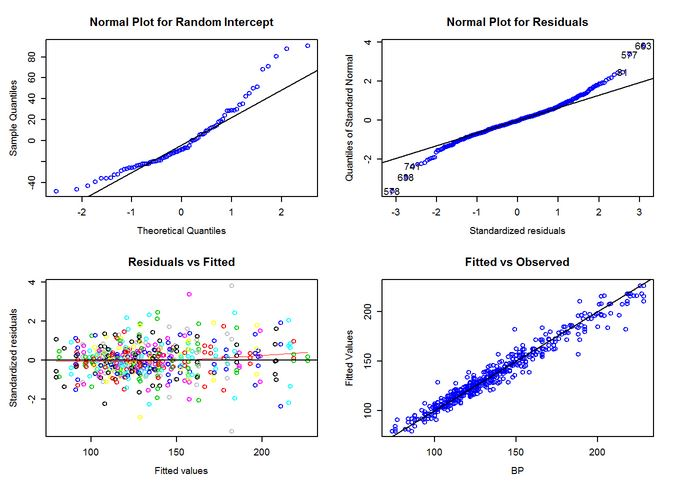
\includegraphics[width=0.9\linewidth]{images/ResidPlot}
	\caption{}
	\label{fig:ResidPlot}
\end{figure}


% Points are labelled by subjects, with cases 67, 68 and 71 being among the prominent cases. 
% Prominent cases warrant further investigation, but an analyst should procede to influence diagnostics beforehand.

% As the LME model can be tailored to the needs of the particular research question, the rationale behind the model appraisal must 
% follow accordingly. 

For method comparison studies, one should create plots specific to each method, useful in determining which methods disagree with the rest.

Figure~\ref{bloodnlme-ResidPlot} depicts residual plot for the Systolic Blood Pressure example, panelled by the various measurement methods, confirming agreement between methods J and R. Lack of agreement between those two methods and method S is also indicated. However, little insight can be gained as to what actually causes this lack of agreement. 
\begin{figure}[h!]
	\centering
	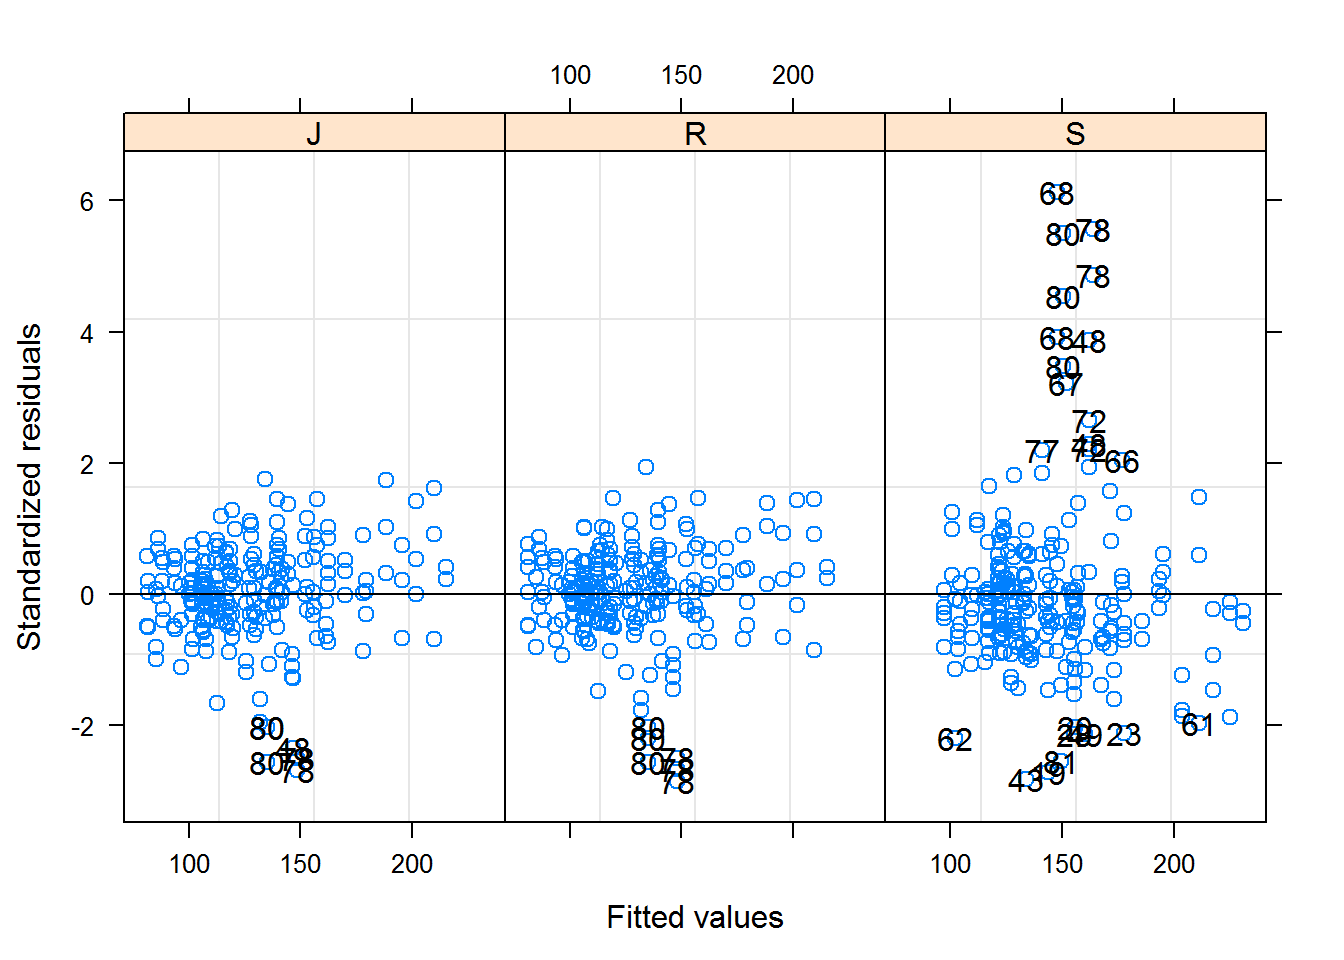
\includegraphics[width=0.8\linewidth]{images/bloodnlme-ResidPlot}
	\caption{LME Residuals by Method (Blood Pressure Data)}
	\label{bloodnlme-ResidPlot}
\end{figure}



%\begin{figure}[h!]
%\centering
%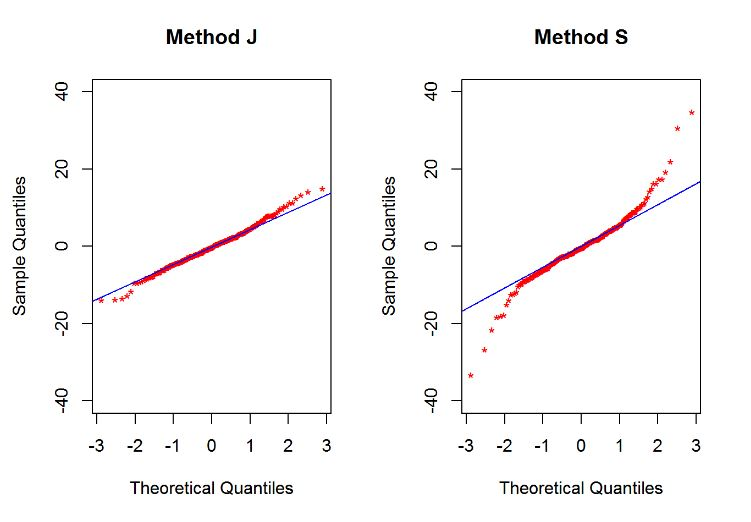
\includegraphics[width=1.1\linewidth]{images/Resid-newplot2}
%\caption{}
%\label{fig:Resid-newplot2}
%\end{figure}


%The fitted model used in the Blood data example, \texttt{JS.ARoy20091}, was fitted using the \texttt{lme()} function from the nlme package, and as such, is stored as an \texttt{lme} object. The \texttt{residual} functions extracts residuals of a fitted LME model, depending on the type of residual required.
%


% \subsubsection{LME Residuals}
% LME are flexible tools for the analysis of clustered and repeated measurement data. LME extend the capabilities of standard linear models by % allowing unbalanced and missing data, as long as the missing data are MAR. Structured covariance matrices for both the random effects G and % the residuals R. 



\subsubsection{Taxonomy of LME Residuals}
Standard residual and influence diagnostics for linear models can
be extended to linear mixed models. The dependence of
fixed-effects solutions on the covariance parameter estimates has
important ramifications in perturbation analysis. To properly assess the
full impact of a set of observations on the analysis, covariance
parameters need to be updated, which requires refitting of the
model.
%---http://www.stat.purdue.edu/~bacraig/notes598S/SUGI_Paper_Schabenberger.pdf

\citet{PB} describes three types of residual that describe the variabilities
present in LME models, marginal residuals which predict marginal errors, conditional residual, which predict conditional errors, and the BLUP, $ {Z\hat{b}}$, that predicts random effects. Each type of residual is useful to evaluates some assumption of the model.

The conditional (subject-specific) and marginal (population-averaged) formulations in the linear mixed model enable you to consider conditional residuals that use the estimated BLUPs of the random effects, and marginal residuals which are deviations from the overall mean. The definitions of both marginal residuals ($r_m$) and conditional residuals ($r_c$) follow from the definitions of marginal and conditional means in the LME model 
$E[{Y}] = {X}{\beta}$ and $E[{Y|{u}}] = {X}{\beta} + {Z}{u}$, respectively.

A marginal residual is the difference between the observed data and the estimated marginal mean, i.e. $r_{Mar} = y - X \hat{\beta}$. A conditional residual is the difference between the observed data and the predicted value of the observation. 
Conditional residuals include contributions from both fixed and random effects, whereas marginal residuals include contribution from only fixed effects. Marginal residuals should have mean of zero, but may show grouping structure. Also they may not be homoscedastic. In a model without random effects, both sets of residuals coincide.



Residuals using the BLUPs are useful to diagnose whether the random effects components in the model are specified correctly, marginal residuals are useful to diagnose the fixed-effects components.

%- http://www.ime.usp.br/~jmsinger/MAE5705/EMR2013.pdf

According to \citet{hilden1995}, a residual is considered pure for a specfic type of error if it depends only on the fixed components and on the error that it is supposed to predict. Residuals that depend on other types of error are known as `confounded errors'.





%In linear mixed effects models, diagnostic techniques may consider `conditional' residuals. A conditional residual is the difference between an observed value $y_{i}$ and the conditional predicted value $\hat{y}_{i} $.
%
%\[ \hat{epsilon}_{i} = y_{i} - \hat{y}_{i} = y_{i} - ( X_{i}\hat{beta} + Z_{i}\hat{b}_{i}) \]
%



%==========================================================================%
\section{Influence Diagnostics}
Model diagnostic techniques can determine whether or not the distributional assumptions are satisfied, but also to assess the influence of unusual observations. Following model specification and estimation, it is of interest to explore the model-data agreement by raising pertinent questions. 

\citet{west} remarks that influence diagnostics play an important role in the interpretation of results, because influential data can negatively influence the statistical model and generalizability of the model. 


Unfortunately this aspect of LME theory is not as expansive as the corresponding body of work for classical linear models. \citet{PB} provide some insight into how to compute and interpret model diagnostic plots for LME models. Their particular observations will be reverted to shortly. 


Influence diagnostics are formal techniques that allow the identification observation that heavily influence estimates of the estimates of fixed effects and variance covariance parameters.


Influential points are a set of one or more observations whose removal would cause a different conclusion in the analysis, e.g. substantially affect estimates. 
Influential points have a large influence on the fit of the model. Influential points are a set of one or more observations whose removal would cause a different conclusion in the analysis, e.g. substantially changes the estimate of the regression coefficients. 




The process of carrying out model diagnostic involves several informal and formal techniques, which will mentioned throughout the chapter.




One approach for determining influential points is to compare the fit of the model with and without each observation. The basic rationale behind identifying influential data is that when iteratively single units are omitted from the data, models based on these data should not produce substantially different estimates. 


\subsection*{Procedure for Quantifying Influence}






\citet{schabenberger} describes a simple procedure for quantifying influence for LME Models. Firstly a model should be fitted to the data, and estimates of the parameters should be obtained. 

The second step is that either single or multiple data points, specifically outliers, should be omitted from the analysis, with the original parameter estimates being updated. This is known as \textit{``leave one out"} or \textit{``leave k out"} analysis. 

The final step of the procedure is comparing the sets of estimates computed from the entire and reduced data sets to determine whether the absence of observations changed the analysis. 


%http://support.sas.com/documentation/cdl/en/statug/63033/HTML/default/viewer.htm#statug_mixed_sect024.htm

%http://www.itl.nist.gov/div898/handbook/pmd/section4/pmd44.htm
\subsection{Comparing Influence and Residual Analysis}
%In LME models, there are two types of residuals, marginal residuals and conditional residuals. A
%marginal residual is the difference between the observed data and the estimated marginal mean. A conditional residual is the
%difference between the observed data and the predicted value of the observation. In a model without random effects, both sets of residuals coincide \citep{schab}.

\citet{influenceLME4} compares residual analysis and influence analysis. Cases with high residuals (defined as the difference between the observed and the predicted scores on the dependent
variable) or with high standardized residuals (defined as the residual divided by the standard deviation
of the residuals) are indicated as outliers.

However, an influential case is not necessarily an outlying residual. On the contrary: a strongly influential case dominates
the regression model in such a way, that the estimated regression line lies closely to this case. The analysis of residuals cannot be used for the detection of influential cases \citep{crawley2012r}.







\subsection*{Case Deletion}

The impact of an observation on a regression fitting can be determined by the difference between the estimated regression coefficient of a model with all observations and the estimated coefficient when the particular observation is deleted. 

The subscript $(U)$ is used to denote quantities computed from data with subset of cases $U$ omitted.
If the global measure suggests that the points in $U$ are influential, you should next determine the nature of
that influence. In particular, the points can affect the estimates of the precision of the fixed effects and covariance parameters, and hence predicted values.


For case-deletion approaches, \citet{preisser} describes two type of diagnostics. When the set consists of only one observation, the type is called
`\textit{observation-diagnostics}'. For multiple observations, Preisser describes the diagnostics as `\textit{cluster-deletion}' diagnostics. Consideration of how leave-$U$-out diagnostics would work in the context of Method Comparison problems is required.  Suppose we have two methods of measurement X and Y, each with three measurements for a specific case: $(x_1,x_2,x_3,y_1,y_2,y_3)$

\begin{itemize}
	\item \textbf{Leave One Out} - one observation is omitted (e.g. $x_1$)
	\item \textbf{Leave Pair Out} - one pair of observation  is omitted (e.g. $x_1$ and $y_1$)
	\item \textbf{Leave item) Out} - All observations associated with a particular case or subject are omitted. (e.g. $\{x_1,x_2,x_3,y_1,y_2,y_3\}$)
\end{itemize}
%% Schabenberger

The natural sampling unit is the item or subject, similar to the example provided by \citet{schabenberger}. Hence, the third option, henceforth, referred to as ``\textit{Leave item out}" will be the option used.

\subsection{Analyzing Influence in LME Models}







Influence can be thought of as consequence of leverage and outlierness. Outliers are the most noteworthy data points in an analysis, and an objective of influence analysis is how influential they are, and the manner in which they are influential. They can point to a model breakdown and lead to development of a better model.

While linear models and GLMS can be studied with a wide range of well-established diagnostic technqiues, the choice of methodology is much more restricted for the case of LMEs. However
influence diagnostics for LME Models is an area of active research. Research on diagnostic analyses for LME models are presented in \citet{Beckman}, 
\citet{Christensen}, \citet{hilden1995}, \citet{lesaffre1998local}, \citet{Banerjee1997}, 
\citet{fung2002}, \citet{Demi}, \citet{Zewotir} and \citet{NobreSinger2007, NobreSinger2011}.

%%- \citet{Hildon 1995}
%%- FIX : Banerjee1997

%%%%%%%%%%%%%%%%%%%%%%%%%%%%%%%%%%%%%%%%%%%%%%%%%%%%%%%%%%%%%%%%%%%%%%%%%%

\citet{schabenberger} states that goal of influence analysis is not primarily to mark data points for deletion so that a better model fit can be achieved for the reduced data, although this might be a result of influence analysis. The goal is rather to determine which cases are influential and the manner in which they are important to the analysis. 



%For example, you are not only concerned with capturing the fixed and random components of the model. The LME model structure presents unique and interesting challenges that prompt us to reexamine the traditional ideas of influence and residual analysis.

%Influence arises at two stages of the LME model. Firstly when $V$ is estimated by $\hat{V}$, and subsequent
%estimations of the fixed and random regression coefficients $\beta$ and $u$, given $\hat{V}$.
%
%Diagnostic methods for fixed effects are generally analogues of methods used in classical linear models.
%Diagnostic methods for variance components are based on `one-step' methods. 



\subsection{Measuring of Influence for LME Models}
%- (Zewotir) 
Influence analysis methodologies have been used extensively in classical linear models, and provided the basis for methodologies for use with LME models. Computationally inexpensive diagnostics tools have been developed to examine the issue of influence \citep{Zewotir}. 

\citet{Zewotir} lists several established methods of analyzing influence in LME models. These methods include Cook's distance for LME models,
\index{likelihood distance} likelihood distance,
the variance (information) ration,
the \index{Cook-Weisberg statistic} Cook-Weisberg statistic, and
the \index{Andrews-Prebigon statistic} Andrews-Prebigon statistic.



\citet{Zewotir} remarks the development of efficient computational formulas is crucial making deletion diagnostics useable, allowing one to obtain the \index{case deletion diagnostics} case deletion diagnostics by making use of basic building blocks, computed only once for the full model. A number of approaches to model diagnostics are described, including variance components, dixed effects parameters, prediction of the response variable and of random effects, and the likelihood function. Influence statistics can be grouped by the aspect of estimation that is their primary target:
\begin{itemize}
	\item \textbf{Overall measures compare changes in objective functions}: (restricted) likelihood distance (Cook and Weisberg 1982, Ch. 5.2)
	\item \textbf{Influence on parameter estimates}: Cook's  (Cook 1977, 1979), MDFFITS (Belsley, Kuh, and Welsch 1980, p. 32)
	\item \textbf{Influence on precision of estimates}: CovRatio and \texttt{},       item \textbf{Influence on fitted and predicted values}: PRESS residual, PRESS statistic (Allen 1974), DFFITS (Belsley, Kuh, and Welsch 1980, p. 15),
	\item \textbf{Outlier properties}: internally and externally studentized residuals, leverage
\end{itemize}




For example, if observations primarily affect the precision of the covariance parameters without exerting much influence on the fixed effects, then their presence in the data may not distort hypothesis
tests or confidence intervals about $\beta$. 
\citet{schabenberger} notes that removing observations or sets of observations affects fixed effects and covariance parameter estimates.





\section{Deletion Diagnostics}

%Data from single individuals, or a small group of subjects may influence non-linear mixed effects model selection. 
%Diagnostics routinely applied in model building may identify such individuals, but these methods are not specifically designed for that purpose and are, therefore, not optimal. 
%We describe two likelihood-based diagnostics for identifying individuals that can influence the choice between two competing models.

Deletion diagnostics provide a means of assessing the influence of an observation (or groups of observations) on parameters inferences for a fitted model. For classical linear models, \citet{cook77} greatly expands the study of residuals and influence measures. The key to making deletion diagnostics useable is the development of efficient computational formulas, allowing one to obtain the \index{case deletion diagnostics} case deletion diagnostics by making use of basic building blocks, computed only once for the full model.


Cook's key observation was the effects of deleting each observation in turn could be calculated with little additional computation. Cook proposed a measure that combines the information of leverage and residual of the observation, now known simply as the Cook's Distance, $D_{(i)}$, which can be calculated without fitting a new regression coefficient each time an observation is deleted. Consequently deletion diagnostics have become an integral part of assessing linear models.

The effect on the precision of estimates is separate from the effect on the point estimates. Data points that have a small \index{Cook's distance}Cook's distance, for example, can still greatly affect hypothesis tests and confidence intervals, if their influence on the precision of the estimates is large.


\citet{Christensen} notes the case deletion diagnostics techniques have not been applied to linear mixed effects models and seeks to develop methodologies in that respect. \citet{Christensen} developed their global influences for the deletion of single observations in two steps: a one-step estimate for the REML (or ML) estimate of the variance components, and an ordinary case-deletion diagnostic for a weighted resgression problem (conditional on the estimated covariance matrix) for fixed effects.


Calculation of case deletion diagnostics in the OLS model is made simple by the fact that estimates of $\beta$ and $\sigma^2$, which exclude the $i$th observation, can be computed without re-fitting the model. Such update formulas are available in the LME model only if you assume that the covariance parameters are not affected by the removal of the observation in question. This is rarely a reasonable assumption, and fundamentally undermines the use of many proposed procedures for method comparison.



\subsection{Cook's Distance}

\index{Cook's Distance} Cooks Distance ($D_{i}$) is a diagnostic technique used in classical linear models, that functions as an overall measure of influence of a subset of observations $U$ on the regression coefficients, and consequently the fitted values. \index{Cook's distance} Cook's Distance as a measure of the influence of observations in subset $U$ on a vector of parameter estimates is given below \citep{cook77}
\[ \delta_{(U)} = \hat{\beta} - \hat{\beta}_{(U)}.\]
Observations, or sets of observations, that have high Cook's distance usually have high residuals, although this is not necessarily the case.


If the predictions are the same with or without the observation in question, then the observation has no influence on the regression model. If the predictions differ greatly when the observation is not included in the analysis, then the observation is influential.

Cook's distance can be used in several ways: to indicate data points that are particularly worth checking for validity; to indicate regions of the design space where it would be good to be able to obtain more data points.


%However, informal heuristics do exist for OLS models, with an informal threshold of $4/n$ or $4/(n-k-1)$, where $n$ is the number of observations and $k$ the number of explanatory variables.
Large values for Cook's distance indicate observations for special attention. Although informal heuristics exist, use of threshold values for Cook's Distance is discouraged \citep{fox1991}. \citet{fox1991} advises the use of diagnostic plotting and to examine in closer details the points with \textit{``values of D that are substantially larger than the rest}", and that thresholds should feature only to enhance graphical displays.

The effect on the precision of estimates is separate from the effect on the point estimates. Data points that have a small \index{Cook's distance}Cook's distance, for example, can still greatly affect hypothesis tests and confidence intervals, if their  influence on the precision of the estimates is large.

\citet{Christensen} develops \index{case deletion diagnostics} case deletion diagnostics, in particular the equivalent of \index{Cook's distance} Cook's distance for diagnosing influential observations when estimating the fixed effect parameters and variance components, adapting the \index{Cook's distance}Cook's Distance measure for the analysis of LME models. 

For LME models, two formulations exist; a \index{Cook's distance}Cook's distance that examines the change in fixed fixed parameter estimates, and another that examines the change in random effects parameter estimates. The outcome of either Cook's distance is a scaled change in either $\beta$ or $\theta$. \citet{Zewotir} gives a detailed discussion of the various formulation for Cook's distances for LME Models.

Such update formulas are available in the LME model only if one can assume that the covariance parameters are not affected by the removal of the observation in question. This is rarely a reasonable assumption, and fundamentally undermines the use of many proposed procedures for method comparison.


%For LME models, Cook's distance can be extended to model influence diagnostics by defining:
%\[ C_{\beta i} = {(\hat{\beta} - \hat{\beta}_{[i]})^{T}(\boldsymbol{X}^{\prime}\boldsymbol{V}^{-1}\boldsymbol{X}) (\hat{\beta} - \hat{\beta}_{[i]}) \over p}\]
%
%It is also desirable to measure the influence of the case deletions on the covariance matrix of $\hat{\beta}$.

%It uses the same structure for measuring the combined impact of the differences in the estimated regression coefficients when the $i$th case is deleted. Importantly, $D_{(i)}$ can be calculated without fitting a new regression coefficient each time an observation is deleted.

%Cook's Distance is proportional to the sum of the squared differences between predictions made with all observations in the analysis and predictions made leaving out the observation in question.


\begin{figure}[h!]
	\centering
	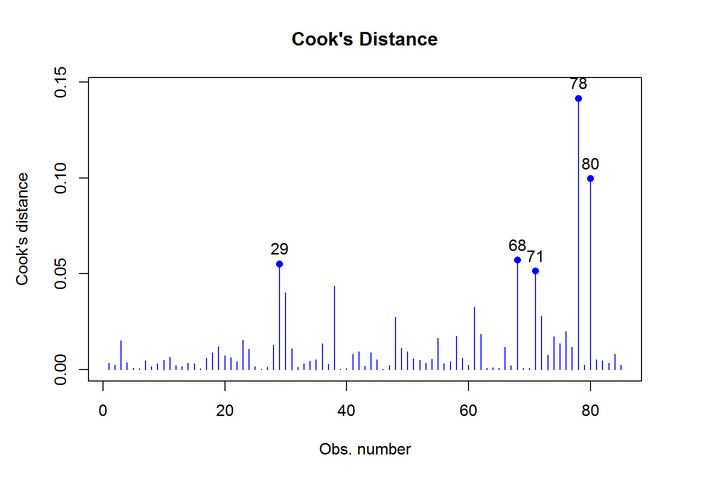
\includegraphics[width=0.9\linewidth]{images/CooksDistancePlot-JS-Roy}
	\caption{}
	\label{fig:CooksDistancePlot-JS-Roy}
\end{figure}
%For LME models, Cook's distance can be extended to model influence diagnostics by defining:
%\[ C_{\beta i} = {(\hat{\beta} - \hat{\beta}_{[i]})^{T}(\boldsymbol{X}^{\prime}\boldsymbol{V}^{-1}\boldsymbol{X}) (\hat{\beta} - \hat{\beta}_{[i]}) \over p}\]
%
%It is also desirable to measure the influence of the case deletions on the covariance matrix of $\hat{\beta}$.
\citet{Christensen} notes the case deletion diagnostics techniques have not been applied to LME models and seeks to develop methodologies in that respect. \citet{Christensen} developed their global influences for the deletion of single observations in two steps: a one-step estimate for the REML (or ML) estimate of the variance components, and an ordinary case-deletion diagnostic for a weighted regression problem (conditional on the estimated covariance matrix) for fixed effects.








\subsection{Local Influence}
\citet{cook86} gives a completely general method for assessing the influence of local departures from assumptions in statistical models, introducing methods for local influence assessment for classical linear models. These methods provide a powerful tool for examining perturbations in the assumption of a model, particularly the effects of local perturbations of parameters of observations. The local-influence approach to influence assessment is quite different from the case deletion approach, comparisons are of interest.

% % Beckman, Nachtsheim and Cook (1987)
\citet{Beckman} applied the \index{local influence}local influence method of Cook (1986) to the analysis of the LME model. Other authors such as \citet{lesaffre1998local} have also extended these idea to LME models. 


While the concept of influence analysis is straightforward, implementation in LME models is more complex. Update formulae for fixed effects models are available only when the covariance parameters are assumed to be known. As such the local influence approach are not particularly useful in the context of method comparison, and so will not be considered further.







\subsection{Iterative and Non-Iterative Influence Analysis}



%----schabenberger page 8
For linear models, the implementation of influence analysis is straightforward, but for LME models the process is more complex. \citet{schabenberger} examines the use and implementation of
influence measures in LME models. \citet{schabenberger} highlights some of the issue regarding implementing LME model diagnostics, describing  the choice between \index{iterative influence analysis} iterative influence analysis and \index{non-iterative influence analysis} non-iterative influence analysis.
\citet{schabenberger} considers several important aspects of the use and implementation of influence measures in LME models, noting that it is not always possible to
derive influence statistics necessary for comparing full- and reduced-data parameter estimates. Closed-form expressions for computing the change in important model quantities might not be available.

\citet{schabenberger} describes the scenario wherein a data point is removed and the new estimate of the $G$ matrix is not positive definite. This may occur if a variance component
estimate now falls on the boundary of the parameter space \citep{schabenberger}. 

%%Non-Iterative
For classical linear models, it is not necessary to refit the model after removing a data point in order to measure the impact of an observation on the model. The change in fixed effect estimates, residuals, residual sums of squares, and the variance-covariance matrix of the fixed effects can be computed based on the fit to the full data alone, using update formulas \citep{sherman, hager1989}.


However, in LME models several important complications arise. Data points can affect not only the fixed effects but also the covariance parameter estimates on which the fixed-effects estimates depend. However update formulas are available only if one assumes that the covariance parameters are not affected by the removal of the observation in question. However, this is rarely a reasonable assumption.
For LME models, non-iterative methods are computationally efficient, but require the rather strong assumption that all covariance parameters are known, and thus are not updated, with the exception of the profiled residual variance.

Update formulas for ``\textit{leave-U-out}" estimates typically fail to account for changes in covariance parameters.  As the influence that each item would have on the variance estimate of a method comparison model is crucial, this substanitally negates their usefulness for Roy's Model.

Iterative influence diagnostics requiring fitting the model without the observations in question. Computation time is substantially longer, although this is balanced by algorithmic simplicity, with no assumptions beyond those used for the original model. A measure of total influence requires updates of all model parameters. This can only be achieved in general is by omitting observations or cases, then refitting the model. 


An iterative analysis may seem computationally expensive. Computing iterative influence diagnostics for $n$ observations requires $n+1$ mixed models to be fitted iteratively.
The execution times for iterative procedures are longer relative to non-iterative procedures, but are not so long that they would dissuade an analyst from using them.
Despite the addition execution time of iteratives
approaches, they are preferable for method comparison problems, as they can facilitate several complementary analyses concurrently. 

Iterative methods retain the potential for useful analyses, if applied at different stage of the modelling process. Diagnostic measures, specifically the DFBETA, have characteristics that would make them very useful at the exploratory stage of the method comparison process. Implicitly various assumptions about variance are used, but simultaneously an approach based on DFBETA can be used to assess if these assumptions are valid.




\subsection{Likelihood Distance}
In LME models fit by
\index{maximum likelihood} maximum likelihood (ML) or \index{restricted maximum likelihood} restricted maximum likelihood (REML), an overall influence measure is the \index{likelihood distance} likelihood distance \citep{CookWeisberg}.

\citet{west} examines a group of methods that examine various aspects of influence diagnostics for LME models. For overall influence, the most common approaches are the \textit{likelihood distance} and the \textit{restricted likelihood distance}.
The \index{likelihood distance} likelihood distance is a global summary measure that expresses the joint influence of the subsets of observations, $U$, on all parameters that were subject to updating. \citet{schabenberger} points out that the likelihood distance $LD(\psi_{(U)})$ is not the log-likelihood obtained by fitting the model to the reduced data set. Instead it is obtained by evaluating the likelihood function based on the full data set (containing all $n$ observations) at the reduced-data estimates.




%==========================================================%
%\subsubsection{Likelihood Distances}

The
procedure requires the calculation of the full data estimates
$\hat{\psi}$ and estimates based on the reduced data set
$\hat{\psi}_{(U)}$. The likelihood distance is given by
determining
\[
LD_{(U)} = 2\{l(\hat{\psi}) - l( \hat{\psi}_{(U)}) \}\]\[
RLD_{(U)} = 2\{l_{R}(\hat{\psi}) - l_{R}(\hat{\psi}_{(U)})\}
\]
Large values indicate that ${\hat{\theta}}$ and ${\hat{\theta}_\omega}$ differ considerably.



%For noniterative methods the following computational devices are used to compute (restricted) likelihood distances provided that the residual variance
%$\sigma^2$ is profiled.



\addcontentsline{toc}{section}{Bibliography}
\bibliographystyle{chicago}
\bibliography{2017bib}
\end{document}


